\documentclass[12pt]{article}
\usepackage{fullpage,psfrag,amsmath,verbatim}
\usepackage[small,bf]{caption}

\usepackage{algorithm, algorithmic, amsfonts, amsmath, amssymb, amsthm, graphicx, url}

\usepackage[utf8]{inputenc}
\usepackage{color}
\usepackage[colorlinks,linkcolor=blue,citecolor=red]{hyperref}

\newcommand{\eq}[1]{\eqref{eq:#1}}
\newcommand{\eqd}[1]{\eqref{eq:#1}}
\newcommand{\fig}[1]{Figure~\ref{fig:#1}}

\newtheorem{theorem}{Theorem}[section]
\newtheorem{lemma}[theorem]{Lemma}
\newtheorem{proposition}[theorem]{Proposition}
\newtheorem{corollary}[theorem]{Corollary}
\newtheorem{question}[theorem]{Question}
\newtheorem{result}[theorem]{Result}

\newtheorem{definition}[theorem]{Definition}
\newtheorem{example}[theorem]{Example}
\newtheorem{remark}[theorem]{Remark}
\numberwithin{equation}{section}

\newcommand{\submit}[2]{\iftoggle{submit}{#1}{#2}}

% math macros
\newcommand{\R}{\mathbb{R}}  
\newcommand{\E}{\mathbb{E}}
\newcommand{\minimize}{\mathrm{minimize}}
\newcommand{\maximize}{\mathrm{maximize}}
\newcommand{\st}{\mathrm{subject to}}

\usepackage{listings}
\definecolor{dkgreen}{rgb}{0,0.6,0}
\definecolor{gray}{rgb}{0.5,0.5,0.5}
\definecolor{mauve}{rgb}{0.58,0,0.82}
\lstset{frame=tb,
  language=Python,
  aboveskip=3mm,
  belowskip=3mm,
  showstringspaces=false,
  columns=flexible,
  basicstyle={\small\ttfamily},
  numbers=none,
  numberstyle=\tiny\color{gray},
  keywordstyle=\color{blue},
  commentstyle=\color{dkgreen},
  stringstyle=\color{mauve},
  breaklines=true,
  breakatwhitespace=true,
  tabsize=3
}

\title{Amplification Factor - AF Score}
\author{{\bf Tuan Tran}}
%\date{} % Activate to display a given date or no date (if empty),
         % otherwise the current date is printed 

\begin{document}
\maketitle
\paragraph{Giới Thiệu} Trong tài liệu này sẽ giới thiệu định nghĩa, ý tưởng và giải thích các scripts dùng để tính toán điểm Amplification Factor (AF) score.

\section{Giới Thiệu về AF score}

\paragraph{Định Nghĩa} AF score được dùng để đo lường sức ảnh hưởng của một người đối với những người khác. Trong dự án Advosight, AF score cụ thể đo lường sức ảnh hưởng của một người dùng facebook đối với mạng xã hội facebook, để có thể thấy được sức ảnh hưởng của người đó. Người dùng có ảnh hưởng có thể đem lại hiệu quả lớn cho các doanh nghiệp và xã hội. Việc xác định được những người có ảnh hưởng giúp các doanh nghiệp xác định được chiến lược truyền thông thông tin một cách hiệu quả nhất. Sức ảnh hưởng của một người được chia ra làm ba loại

\begin{itemize} 

\item{Người có ảnh hưởng chung trên mạng xã hội (Celebrity):} Những người có uy tín nhất định đối với cộng đồng hay xã hội, như các diễn viên, ca sĩ, người mẫu trong các lĩnh vực nghệ thuật, thường đưa ra các quan điểm hay nhận xét về 1 sự kiện hay sự vật trên các mạng xã hội. Họ có khả năng tác động nhất định đối với cộng đồng và xã hội.


\item{Người có ảnh hưởng trên một ngành hàng/lĩnh vực kinh doanh (Micro Influencer):} Tương tự như những người ảnh hưởng chung trên mạng xã hội, trong một ngành hàng hay lĩnh vực kinh doanh cũng có những người có uy tín nhất định, thường là các chuyên gia, các nhà nghiên cứu hay là những người chuyên dùng thử. Họ thường đưa ra các ý kiến, các nhận xét cũng như đánh giá về một lĩnh vực hay ngành hàng mà họ có sự hiểu biết và kiến thức. Họ sẽ có tác động nhất định đối với những người tiêu dùng hay khách hàng trong ngành hàng đó.

\item{Người có ảnh hưởng đối với một thương hiệu:} Những người có uy tín nhất định, và tình cảm nhất định đối với 1 thương hiệu nào đó. Những người này thường có xu hướng biểu đạt các nhận xét và đánh giá về các sản phẩm cho thương hiệu mà họ yêu thích hay không thích.

\end{itemize}


\paragraph{Phương pháp tiếp cận} Để xác định tầm ảnh hưởng của một người dùng, trước tiên chúng tôi phải xây dựng mô hình ontology để biểu diễn các mối quan hệ giữa các người dùng trên mạng xã hội. Trên mô hình mạng xã hội đó, chúng tôi sẽ đánh giá tầm ảnh hưởng của người dùng dựa trên số lượng tương tác. Tầm ảnh hưởng của một người được xác định bằng số lượng người tương tác với một ý kiến, nhận xét của của người đó trên mạng xã hội trong một khoảng thời gian nhất định. Sự tương tác có thể được hiểu rằng người tiếp nhận thông tin đã bị ảnh hưởng bởi người đưa ra ý kiến hay quan điểm. Sự ảnh hưởng được chia làm 2 loại: sức ảnh hưởng của một bài đăng và sức ảnh hưởng của người dùng.

\begin{itemize} 

\item Sức ảnh hưởng của một bài đăng được tính bằng tổng số người tương tác đối với bài đăng đó mà không trùng nhau.

\item Sức ảnh hưởng của một người sẽ được tính bằng giá trị trung bình của sức ảnh hưởng các bài đăng của người đó trong khoảng thời gian nhất định.

\end{itemize}

\begin{center}
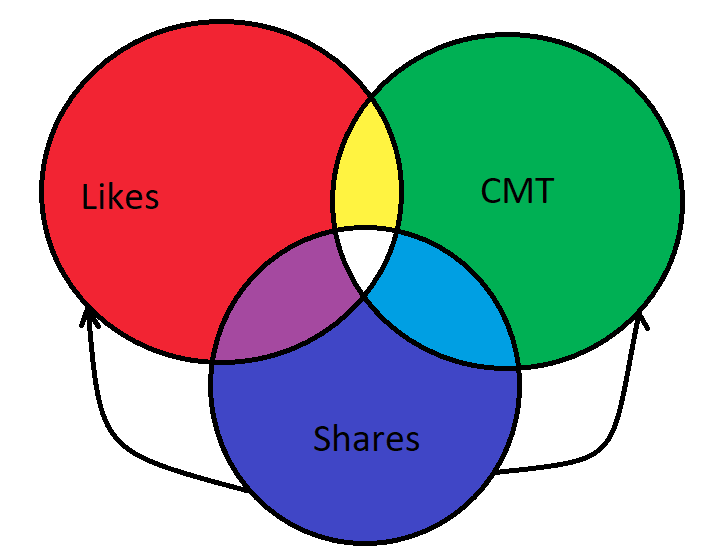
\includegraphics[scale=.5]{hinh_af}
\end{center}
$$
\begin{aligned}
AF ={}{}&|Reactions| + |cmts| + |shares|\\
	  	& - (|reactions \cap cmts| + |cmts \cap shares| + |reactions \cap shares|)\\
		& + |reactions \cap cmts \cap shares|
\end{aligned}
$$

\paragraph{} Như công thức ở trên, thì điểm ảnh hưởng được đo bằng tổng không trùng nhau của số người likes, comments và shares. Trong đó số share là hệ số quang trọng, shares giúp số lượng tương tác của bài gốc tăng lên đáng kể, vì nó làm cho nhiều người khác biết đến một bài đăng có nội dung tốt. Vì vậy từ số lượng tương tác trên những bài shares cũng được tính vào bài gốc.

\section{Diễn giải về script}

\paragraph{} Trước hết cần phải import các library cần thiết đặc biệt là pymongo bởi vì database là MongoDB. Và sau đó là tạo kết nối với database.

\begin{lstlisting}
import pymongo
from pymongo import MongoClient
import datetime
import pandas as pd
import numpy as np
import gc
gc.enable()

client_1 = MongoClient('45.122.223.198:27017',        	#IP address of database
                    username = 'kapiReadOnly', 			#Username
                    password = 'pl2oieAt9#tnWV!Yc0',    #Password
                    authSource = 'kapi',                #name of database
                    authMechanism = 'SCRAM-SHA-1'
                    )
database_1 = client_1['kapi']

\end{lstlisting}

\paragraph{} Bước tiếp theo là tạo các function để query data từ database. Sẽ có 3 functions để liên quang nhau để có thể query và aggregate data cần thiết. Function đầu tiên là các id của bài post, query tất cả những người đã tương tác (likes, comments và shares) với bài post đó từ các bảng 'reactions', 'comments', 'posts', sẽ trả ra 3 bảng lần lượt là tb1, tb2 và tb3. Ba bảng này sẽ được dùng để tính distinct sum của các lượt tương tác về sau.
\\

\begin{lstlisting}
def int_fun(post_id):
    cluster1 = database_1['reactions'].find({'fid': {'$in': post_id}},
                                            {'_id': 0, 'fid': 1, 'from_user_id': 1})
    cluster2 = database_1['comments'].find({'post_id': {'$in': post_id}},
                                           {'_id': 0, 'post_id': 1, 'from_raw_user': 1, 'from_user': 1})
    cluster3 = database_1['posts'].find({'parent_id': {'$in': post_id}},
                                        {'_id': 0, 'parent_id': 1, 'from_user': 1, 'comments_count': 1,
                                         'likes_count': 1})

    tb1 = pd.DataFrame()
    for a in cluster1:
        tmp = pd.DataFrame([a])
        tb1 = tb1.append(tmp, ignore_index=True)

    tb2 = pd.DataFrame()
    for b in cluster2:
        tmp = pd.DataFrame([b])
        tb2 = tb2.append(tmp, ignore_index=True)

    tb3 = pd.DataFrame()
    for c in cluster3:
        tmp = pd.DataFrame([c])
        tb3 = tb3.append(tmp, ignore_index=True)

    for i in range(len(tb2)):
        if tb2.from_user[i] == '':
            tb2.from_user[i] = tb2.from_raw_user[i]

    return tb1, tb2, tb3
\end{lstlisting}

\paragraph{} Function thứ hai được dùng để gọi các thông tin cần thiết khác từ các id của bài posts.
\\

\begin{lstlisting}
def info_fun(fid_list):
    cluster = database_1['posts'].find({'fid': {'$in': fid_list}},
                                       {'_id': 0, 'fid': 1, 'to_user': 1, 'created_date': 1,
                                        'comments_count': 1, 'shares_count': 1, 'likes_count': 1})

    info_tb = pd.DataFrame()
    for i in cluster:
        tmp = pd.DataFrame([i])
        info_tb = info_tb.append(tmp, ignore_index=True)

    return info_tb
\end{lstlisting}

\paragraph{} Function cuối cùng, cũng là function quan trọng nhất. Trong function này, cần phải khai báo danh sách user cần tính AF, thời gian tính AF score (ngày bắt đầu, ngày kết thúc), speed (thường để là 10 để tránh tình trạng timeout). Function này sẽ sử dụng các function ở trên để query data cần thiết sau đó aggregate cũng như tính toán điểm AF score cho từng bài posts của các user id mà chúng ta cần tính, trong khoảng thời gian đã xác định.
\\
\\
\\
\\
\\
\begin{lstlisting}
def retrieve_fun(id_list, start_date, end_date, speed):
    tab1 = database_1['posts'].find({'to_user': {'$in': id_list},
                                     'created_date': {'$gte': start_date, '$lt': end_date},
                                     }, {
                                        '_id': 0, 'fid': 1
                                    })

    ipt = pd.DataFrame()
    for i in tab1:
        tmp = pd.DataFrame([i])
        ipt = ipt.append(tmp, ignore_index=True)

    print("There are {:} messages for processing .".format(len(ipt)))

    int_tmp = pd.DataFrame()
    cmt_tmp_tb = pd.DataFrame()
    shr_tmp_tb = pd.DataFrame()
    len_tmp = (len(ipt) // speed + 1)

    try:
        for i in range(len_tmp):
            print('==Processing to==> {:.4}%'.format(((i + 1) * 100) / len_tmp))
            tb1_tmp, tb2_tmp, tb3_tmp = int_fun(ipt['fid'][i * speed:(i + 1) * speed].tolist())
            int_tmp = int_tmp.append(tb1_tmp, ignore_index=True)
            cmt_tmp_tb = cmt_tmp_tb.append(tb2_tmp, ignore_index=True)
            shr_tmp_tb = shr_tmp_tb.append(tb3_tmp, ignore_index=True)
    except pymongo.errors.CursorNotFound:
        print("Lost cursor. Retry with skip")

    cmt_tmp = pd.DataFrame({'fid': cmt_tmp_tb.post_id, 'from_user_id': cmt_tmp_tb.from_user})
    shr_tmp = pd.DataFrame({'fid': shr_tmp_tb.parent_id, 'from_user_id': shr_tmp_tb.from_user})

    shr_tmp_tb['sub score'] = shr_tmp_tb['comments_count'] + shr_tmp_tb['likes_count']
    af_tmp = shr_tmp_tb.groupby('parent_id').agg({'sub score': 'sum'}).reset_index()
    af_tmp.columns = ['fid', 'sub score']

    total_int_tmp = int_tmp.append([cmt_tmp, shr_tmp]).drop_duplicates().reset_index(drop=True)
    total_int_tmp = total_int_tmp.groupby('fid').agg('count')
    total_int_tmp = af_tmp.set_index('fid').join(total_int_tmp, how='right')

    post_query_tmp = info_fun(total_int_tmp.index.tolist())
    post_query_tmp = post_query_tmp.set_index('fid')

    combine_tb = total_int_tmp.join(post_query_tmp)
    combine_tb['AF score'] = [np.nansum([x, y]) for x, y in
                              zip(combine_tb['from_user_id'], combine_tb['sub score'])];

    return combine_tb
\end{lstlisting}

\paragraph{} Phần cuối là các lệnh cần thiết, gọi các function ở trên tính toán. Sau đó là lưu bảng kết quả ra file '.csv'
\\

\begin{lstlisting}
start_date = datetime.datetime(2018,7,1) #Year, Month, Day of start date
end_date = datetime.datetime(2018,12,31)  #Year, Month, Day of end date

r_tb = retrieve_fun(c_list, start_date, end_date, speed=10)

r_tb.to_csv('c_list.csv')
\end{lstlisting}

\paragraph{} Sau khi tính được AF score cho từng bài posts, ta có thể tính điểm AF cho các user trong 1 khoảng thời gian dễ dàng bằng command line sau.

\begin{lstlisting}
af_df = (r_tb
         .groupby(['to_user'])
         .agg({'AF score': 'mean', 'fid':'count'})
         .reset_index()
         .sort_values(['AF score'], ascending=False)
         .rename({'to_user': 'from_user', 'fid': 'count'}, axis='columns'))


af_df.to_csv('af_scr.csv') #save AF score to csv file.
\end{lstlisting}

\nocite{*}
\bibliographystyle{plain}
\bibliography{refLP}

\end{document}
